\documentclass[../structural_economics_book.tex]{subfiles}
\begin{document}
\ifSubfilesClassLoaded{\setcounter{chapter}{0}}{}
\chapter{Economics in Matrix Notation}\label{ch:01}
\chaptersubtitle{The Standard Model, Rewritten So the Structure Becomes Visible}
\begin{quote}
\textit{``La realidad est\'{a} destruyendo en la Am\'{e}rica Latina aquel pret\'{e}rito esquema de la divisi\'{o}n internacional del trabajo que, despu\'{e}s de haber adquirido gran vigor en el siglo XIX, segu\'{i}a prevaleciendo doctrinariamente hasta muy avanzado el presente.''}\\[0.3em]
\textnormal{[``Reality is destroying in Latin America that outdated scheme of the international division of labor which, after acquiring great vigor in the nineteenth century, continued to prevail doctrinally until well into the present.'']}\\
\hfill --- Ra\'{u}l Prebisch, \textit{El desarrollo econ\'{o}mico de la Am\'{e}rica Latina} (1949)
\end{quote}
\nocite{prebisch1949desarrollo}

\begin{quote}
\textit{``The purpose of abstracting is not to be vague, but to create a new semantic level in which one can be absolutely precise.''}\\
\hfill --- Edsger W.\ Dijkstra, \textit{The Humble Programmer} (1972)
\end{quote}
\nocite{dijkstra1972humble}

\vspace{1em}

This chapter does one thing: it rewrites the economics you already know in a notation that reveals the economics you have not been taught.

Every result here is standard. If you have taken intermediate microeconomics, you know the consumer's problem, the producer's problem, and the idea of market equilibrium. If you have taken a first course in linear algebra, you know what a matrix is and how to multiply them. This chapter puts the two together.

The payoff comes at the end. In Section~\ref{ch01:sec:implicit_W}, we will name an object that is present in every microeconomics textbook but that no microeconomics textbook names: the \textit{interaction matrix} --- the mathematical description of how agents in the economy relate to each other. The standard competitive model implies a very specific interaction matrix: anonymous, rank one, with each agent weighted by her wealth share. Structural economics is what happens when you replace that matrix with the one the world actually has --- non-anonymous, with utility interdependence, and with a distribution of power that the network itself produces.

But first, the standard model.


%% =====================================================================
\section{Who Gets What: The Allocation Matrix}
\label{ch01:sec:allocation}
%% =====================================================================

Economics studies how scarce resources are distributed among people. Let us write this down in the simplest possible way.

\subsection{A Small Economy}

Suppose there are 3 people and 2 goods --- call them Food and Clothing. Each person consumes some amount of each good. We can organize this information in a table:

\begin{center}
\begin{tabular}{lcc}
\toprule
& Food & Clothing \\
\midrule
Ana & 4 & 2 \\
Boris & 3 & 5 \\
Carmen & 1 & 3 \\
\bottomrule
\end{tabular}
\end{center}

Ana eats 4 units of Food and wears 2 units of Clothing. Boris eats 3, wears 5. Carmen eats 1, wears 3. This table is the entire economy. Every question economics asks --- Is this allocation efficient? Fair? Sustainable? Better or worse than some alternative? --- is a question about the numbers in this table.

Now write the table as a matrix:
\begin{equation}\label{ch01:eq:X_example}
X = \begin{pmatrix} 4 & 2 \\ 3 & 5 \\ 1 & 3 \end{pmatrix}.
\end{equation}

Each \textit{row} is a person. Each \textit{column} is a good. The entry $X_{i\ell}$ tells us how much of good $\ell$ person $i$ consumes.

\begin{intuition}[Reading the matrix two ways]
Read the matrix by rows and you see individuals: Ana's bundle is $(4, 2)$, Boris's is $(3, 5)$, Carmen's is $(1, 3)$. Read it by columns and you see the distribution of each good: Food is split $(4, 3, 1)$ across three people, Clothing is split $(2, 5, 3)$. The row view is how microeconomics usually thinks --- one person at a time. The column view is how a planner or a sociologist thinks --- one resource at a time, distributed across a population. This book uses both.
\end{intuition}

\begin{definition}[Allocation Matrix]\label{ch01:def:allocation}
For an economy with $N$ agents and $L$ goods, the \textbf{allocation matrix} is the $N \times L$ matrix
\begin{equation}\label{ch01:eq:X}
X = \begin{pmatrix} x_1' \\ x_2' \\ \vdots \\ x_N' \end{pmatrix},
\end{equation}
where $x_i = (x_{i1}, x_{i2}, \ldots, x_{iL})' \in \R^L_+$ is agent $i$'s consumption vector. Row $i$ is person $i$'s bundle. Column $\ell$ is the distribution of good $\ell$ across agents.
\end{definition}

How much Food exists in total? Sum the first column: $4 + 3 + 1 = 8$. In matrix notation: $\ones'X e_1 = 8$, where $\ones = (1, 1, 1)'$ is the vector of ones and $e_1 = (1, 0)'$ picks out the first column.

More generally, the total endowment of each good is the vector $\ones'X$: a $1 \times L$ row vector whose $\ell$-th entry is the total amount of good $\ell$ consumed.


\subsection{Endowments: Where People Start}

Before any trade or production happens, each person starts with some stuff. Ana might have 6 units of Food and 1 of Clothing (she is a farmer). Boris might have 1 of Food and 6 of Clothing (he is a tailor). Carmen might have 1 of each.

\begin{equation}\label{ch01:eq:Omega_example}
\Omega = \begin{pmatrix} 6 & 1 \\ 1 & 6 \\ 1 & 3 \end{pmatrix}.
\end{equation}

The endowment matrix $\Omega$ has the same shape as $X$: $N \times L$. Entry $\omega_{i\ell}$ is how much of good $\ell$ person $i$ starts with. The total supply of each good is $\ones'\Omega$: here, $(8, 10)$ --- 8 units of Food and 10 of Clothing exist in total.

\begin{definition}[Feasibility]\label{ch01:def:feasibility}
An allocation $X$ is \textbf{feasible} if nobody consumes more of any good than exists in total:
\begin{equation}
\ones'X \leq \ones'\Omega \qquad (\text{component-wise for each good}).
\end{equation}
With equality (no waste), this is $\ones'X = \ones'\Omega$: total consumption equals total endowment.
\end{definition}

Check: in our example, $\ones'X = (8, 10)$ and $\ones'\Omega = (8, 10)$. The allocation is feasible.


%% =====================================================================
\section{The Consumer's Problem}
\label{ch01:sec:consumer}
%% =====================================================================

\subsection{What People Want}

Each person has preferences over bundles. Ana might prefer more Food, Boris might prefer more Clothing, Carmen might want a balanced mix. We represent preferences by a utility function $U_i(x_i)$: a number that is higher when person $i$ is happier with her bundle $x_i$.

Each person chooses the bundle that makes her happiest, subject to what she can afford. If prices are $p = (p_F, p_C)' = (1, 2)'$ (Food costs 1, Clothing costs 2), then Ana's budget is $p'\omega_{\text{Ana}} = 1 \cdot 6 + 2 \cdot 1 = 8$ dollars. She can buy any bundle $(x_F, x_C)$ with $x_F + 2x_C \leq 8$.

\begin{definition}[The Consumer's Problem]\label{ch01:def:consumer_problem}
Agent $i$ solves:
\begin{equation}\label{ch01:eq:consumer}
\max_{x_i \geq 0} \; U_i(x_i) \quad \text{subject to} \quad p'x_i \leq p'\omega_i.
\end{equation}
The solution $x_i^*(p, w_i)$ is agent $i$'s \textbf{Marshallian demand}, where $w_i = p'\omega_i$ is her wealth.
\end{definition}

For the entire economy, stack the $N$ problems. Define the wealth vector $\w = \Omega p$: an $N \times 1$ vector whose $i$-th entry is $w_i = p'\omega_i$. The budget constraints become:
\begin{equation}\label{ch01:eq:budget_system}
Xp \leq \Omega p = \w.
\end{equation}

\begin{intuition}[What this equation hides]
Look at equation~\eqref{ch01:eq:consumer} carefully. Agent $i$'s utility depends only on $x_i$ --- her \textit{own} consumption. Nobody else's consumption appears. Ana does not care what Boris eats. Boris does not care what Carmen wears. Each person optimizes in isolation, connected to others only through the price vector $p$.

This is an assumption, not a fact. In the real world, people care intensely about what others consume, earn, and do. The keeping-up-with-the-Joneses effect, peer pressure, status competition, network externalities --- all of these are cases where $U_i$ depends on $x_j$ for $j \neq i$. The standard model assumes all of these away.

We will make this assumption visible and then relax it.
\end{intuition}


\subsection{A Worked Example: Cobb-Douglas}

Suppose all three agents have the same preferences:
\begin{equation}
U_i(x_{i1}, x_{i2}) = x_{i1}^{1/2} \, x_{i2}^{1/2}.
\end{equation}

This is the Cobb-Douglas utility function with equal weights on both goods. The Marshallian demands (derived by setting up the Lagrangian and solving the first-order conditions --- see any intermediate micro text) are:
\begin{equation}\label{ch01:eq:CD_demand}
x_{i1}^* = \frac{w_i}{2p_1}, \qquad x_{i2}^* = \frac{w_i}{2p_2}.
\end{equation}

Each person spends half her income on each good. Let $p = (1, 1)'$ (both goods cost 1). Then:
\begin{align}
w_{\text{Ana}} &= 1 \cdot 6 + 1 \cdot 1 = 7, \\
w_{\text{Boris}} &= 1 \cdot 1 + 1 \cdot 6 = 7, \\
w_{\text{Carmen}} &= 1 \cdot 1 + 1 \cdot 3 = 4.
\end{align}

The demands are:
\begin{equation}
X^* = \begin{pmatrix} 3.5 & 3.5 \\ 3.5 & 3.5 \\ 2.0 & 2.0 \end{pmatrix}.
\end{equation}

\begin{intuition}[Two things to notice]
First, Ana and Boris have \textit{identical demands} even though they start with very different endowments (Ana has mostly Food, Boris has mostly Clothing). The market --- through trade at prices $p$ --- erases the difference. This is the power of markets: they allow people to trade away from their endowments toward their preferred bundles.

Second, Carmen consumes less of \textit{both} goods. Not because she has different preferences (all three have the same $U_i$), but because she is poorer. Her endowment has lower total value. The allocation matrix $X^*$ reflects not just preferences but wealth --- and wealth reflects endowments, which reflect history.

This is the first hint of the structural question: where do the endowments come from?
\end{intuition}

Now write the demand in matrix form. From~\eqref{ch01:eq:CD_demand}, each person's bundle is $x_i^* = \frac{w_i}{2}(1/p_1, 1/p_2)'$. Stack them:
\begin{equation}\label{ch01:eq:CD_matrix}
X^* = \frac{1}{2} \w \cdot (1/p_1, \; 1/p_2) = \frac{1}{2} \begin{pmatrix} 7 \\ 7 \\ 4 \end{pmatrix} \begin{pmatrix} 1 & 1 \end{pmatrix}.
\end{equation}

The allocation matrix is the \textit{outer product} of the wealth vector $\w$ and the price-dependent expenditure-share vector $(1/2p_1, 1/2p_2)$. Every row is a scalar multiple of the same vector. People differ only in \textit{how much} they consume, not in \textit{what} they consume.

\begin{keyinsight}
In the Cobb-Douglas model, the allocation matrix $X^*$ is a \textbf{rank-1 matrix}: it can be written as a column vector times a row vector. Rank 1 means all rows are proportional. This is the mathematical signature of an economy where people differ only in wealth, not in preferences or social position.

When we introduce social structure in Chapter~5, the allocation matrix will have higher rank. Different agents will consume different \textit{kinds} of bundles, not just different \textit{amounts} of the same bundle. The rank of $X$ is a measure of structural differentiation.
\end{keyinsight}


\subsection{Market Clearing: Does Everything Add Up?}

Check feasibility: $\ones'X^* = (3.5 + 3.5 + 2.0, \; 3.5 + 3.5 + 2.0) = (9, 9)$. But total endowment is $\ones'\Omega = (8, 10)$. Food demand exceeds supply by 1; Clothing demand falls short by 1. The allocation is not feasible at these prices.

This means $p = (1, 1)$ is not an equilibrium price. The correct price must adjust to equate supply and demand. We need to find $p^*$ such that $\ones'X^*(p^*) = \ones'\Omega$.

Setting up the market-clearing condition for Food (normalizing $p_1 = 1$):
\begin{equation}
\frac{w_1}{2} + \frac{w_2}{2} + \frac{w_3}{2} = 8 \quad \Rightarrow \quad \frac{(6 + p_2) + (1 + 6p_2) + (1 + 3p_2)}{2} = 8.
\end{equation}

Solving: $\frac{8 + 10p_2}{2} = 8$, so $8 + 10p_2 = 16$, giving $p_2^* = 0.8$.

At $p^* = (1, 0.8)$: $w_{\text{Ana}} = 6.8$, $w_{\text{Boris}} = 5.8$, $w_{\text{Carmen}} = 3.4$. The equilibrium allocation is:
\begin{equation}
X^* = \begin{pmatrix} 3.40 & 4.25 \\ 2.90 & 3.63 \\ 1.70 & 2.13 \end{pmatrix}.
\end{equation}

Verify: column sums are $(8.0, 10.0)$. Markets clear. This is the \textbf{Walrasian equilibrium}.


%% =====================================================================
\section{The One-Good Economy: Welfare and Power}
\label{ch01:sec:one_good}
%% =====================================================================

The multi-good case demonstrates trade. But to see \textit{power} clearly, we need the simplest possible setting: one good, $N$ agents, and the question of who gets how much.

\subsection{Setup}

$N$ agents share a total endowment $\Omega > 0$ of a single good. Person $i$ starts with $\omega_i \geq 0$ and $\sum_i \omega_i = \Omega$. Preferences are quadratic:
\begin{equation}\label{ch01:eq:LQ}
U_i(x_i) = x_i - \frac{\kappa}{2}x_i^2, \qquad \kappa > 0.
\end{equation}

This utility function is concave: the first unit is worth approximately 1, each additional unit is worth less, and the marginal utility hits zero at $x_i = 1/\kappa$. The parameter $\kappa$ controls how fast the returns diminish. Think of it as how quickly a person gets ``full.''

\begin{example}[Three People, One Good]\label{ch01:ex:one_good}
Let $N = 3$, $\kappa = 0.5$, $\Omega = 3$. Endowments: $\omega_1 = 1.8$, $\omega_2 = 0.6$, $\omega_3 = 0.6$. Satiation is at $1/\kappa = 2$, so every allocation considered below satisfies $\kappa x_i < 1$: more is always better.

Person 1 is rich (starts with 1.8 out of 3). Persons 2 and 3 are poor (start with 0.6 each).

\textbf{What is the best possible allocation?} A utilitarian planner maximizes total welfare $\sum_i U_i(x_i)$ subject to $\sum_i x_i = 3$. The first-order conditions require equal marginal utility: $1 - \kappa x_i = 1 - \kappa x_j$, so $x_i = x_j$ for all $i, j$. Equal division: $x_i^{FB} = 1$ for all $i$.

Total welfare at the first-best: $\mathcal{W}^{FB} = 3 \times (1 - 0.25) = 2.25$.

\textbf{What happens without a planner?} With one good there is nothing to trade, so each person consumes her endowment: $x_1 = 1.8$, $x_2 = x_3 = 0.6$.

Welfare: $\mathcal{W}^{0} = (1.8 - 0.81) + 2(0.6 - 0.09) = 0.99 + 1.02 = 2.01$.

The rich person's last units are worth little: her marginal utility is $1 - 0.5 \times 1.8 = 0.1$, while each poor person's is $1 - 0.5 \times 0.6 = 0.7$. Moving a unit from person 1 to person 2 would raise total utility by roughly $0.6$.

\textbf{The welfare loss:} $L = \mathcal{W}^{FB} - \mathcal{W}^{0} = 2.25 - 2.01 = 0.24$, about 11\% of first-best welfare. This is a \textit{utilitarian} (distributional) loss: the endowment allocation is Pareto efficient, since any reallocation makes someone worse off.
\end{example}

\begin{proposition}[Welfare Loss from Inequality]\label{ch01:prop:welfare_loss}
In the one-good economy with quadratic utility~\eqref{ch01:eq:LQ}, the welfare loss from endowment inequality is:
\begin{equation}\label{ch01:eq:welfare_loss}
L = \frac{\kappa N}{2} \cdot \text{Var}(\omega_i),
\end{equation}
where $\text{Var}(\omega_i) = \frac{1}{N}\sum_i \omega_i^2 - \left(\frac{\Omega}{N}\right)^2$ is the variance of endowments. The loss is zero if and only if all endowments are equal.
\end{proposition}

\begin{intuition}[What this says in words]
The cost of inequality is proportional to three things: how curved preferences are ($\kappa$), how many people there are ($N$), and how unequally the endowment is distributed ($\text{Var}(\omega_i)$). More curvature means the rich waste more of what they have (diminishing returns bite harder). More people means more total waste. More inequality means more mismatch between who has stuff and who can use it.

This is the simplest possible welfare cost of inequality. In the structural model, the question becomes: where does $\text{Var}(\omega_i)$ come from? The answer will be: from the weight matrix.
\end{intuition}

\begin{proof}
First-best welfare: $\mathcal{W}^{FB} = N \cdot U(\Omega/N) = N[\Omega/N - \frac{\kappa}{2}(\Omega/N)^2] = \Omega - \frac{\kappa\Omega^2}{2N}$.

Endowment welfare: $\mathcal{W}^{0} = \sum_i U_i(\omega_i) = \sum_i[\omega_i - \frac{\kappa}{2}\omega_i^2] = \Omega - \frac{\kappa}{2}\sum_i\omega_i^2$.

The difference:
\begin{equation}
L = \mathcal{W}^{FB} - \mathcal{W}^{0} = \frac{\kappa}{2}\left(\sum_i \omega_i^2 - \frac{\Omega^2}{N}\right) = \frac{\kappa}{2} \cdot N \cdot \text{Var}(\omega_i).
\end{equation}
The last step uses the identity $\sum_i \omega_i^2 - \Omega^2/N = N \cdot \text{Var}(\omega_i)$. Since $\kappa N/2 > 0$, $L = 0$ if and only if $\text{Var}(\omega_i) = 0$, that is, if and only if every $\omega_i = \Omega/N$. (The planner's first-best is equal division because $\sum_i U(x_i)$ is strictly concave and symmetric, so its unique maximizer on $\sum_i x_i = \Omega$ is the symmetric point.)
\end{proof}

\begin{example}[Verifying the Formula]
In Example~\ref{ch01:ex:one_good}: $\text{Var}(\omega) = \frac{1}{3}(3.24 + 0.36 + 0.36) - 1^2 = 1.32 - 1 = 0.32$. So $L = \frac{0.5 \cdot 3}{2} \cdot 0.32 = 0.24$. Matches.
\end{example}


\subsection{Bargaining: When Power Enters}

In a one-good exchange economy there is nothing to bargain over: the endowment allocation is already Pareto efficient. Bargaining needs a \textit{surplus}. So change the story. Agent 1 is a landowner; agents 2 and 3 are laborers. Working together they produce a harvest of $\Omega$; if they fail to agree, each falls back on a disagreement payoff $d_i$ (what the landowner can grow alone, what the laborers earn elsewhere), with $\sum_i d_i < \Omega$. The joint surplus $\Omega - \sum_i d_i$ is what bargaining power divides. Payoffs are in units of the good, so utility is transferable for the purpose of bargaining; we use the concave $U$ in~\eqref{ch01:eq:LQ} only to \textit{evaluate} welfare.

We model the division through the \textbf{generalized (asymmetric) Nash bargaining solution}: the allocation maximizes a weighted product of gains over disagreement.

\begin{definition}[Bargaining Power]\label{ch01:def:bargaining_power}
The \textbf{bargaining weight vector} is $\boldsymbol{\lambda} = (\lambda_1, \ldots, \lambda_N)'$ with $\lambda_i > 0$ and $\sum_i \lambda_i = 1$. Agent $i$'s weight $\lambda_i$ represents her share of total bargaining power.
\end{definition}

\begin{definition}[Nash Bargaining Solution]\label{ch01:def:nash}
The \textbf{Nash bargaining allocation} maximizes:
\begin{equation}\label{ch01:eq:nash}
\max_{\x} \sum_{i=1}^N \lambda_i \ln\bigl(x_i - d_i\bigr) \quad \text{subject to} \quad \sum_i x_i = \Omega, \quad x_i > d_i,
\end{equation}
where $d_i$ is agent $i$'s \textbf{disagreement payoff} --- what she gets if bargaining fails.
\end{definition}

\begin{proposition}[Nash Division of the Surplus]\label{ch01:prop:nash_division}
Let $\lambda_i > 0$ for all $i$ and $\Omega > \sum_j d_j$. Then~\eqref{ch01:eq:nash} has the unique solution
\begin{equation}\label{ch01:eq:nash_division}
x_i = d_i + \lambda_i\Bigl(\Omega - \sum_{j} d_j\Bigr).
\end{equation}
Every agent receives her disagreement payoff plus a share $\lambda_i$ of the joint surplus. The allocation exhausts the harvest, so it is Pareto efficient for every $\boldsymbol{\lambda}$: in units of the good, and in the utilities $U$ of~\eqref{ch01:eq:LQ} whenever $\kappa x_i \le 1$ for every $i$.
\end{proposition}

\begin{proof}
This is the asymmetric Nash solution \citep{kalai1977nonsymmetric} for transferable utility. The feasible set $\{x : \sum_i x_i = \Omega,\ x_i > d_i\}$ is nonempty because $\Omega > \sum_j d_j$, and the objective is strictly concave on it and tends to $-\infty$ at its boundary, so a maximizer exists, is interior and is unique. The Lagrange condition is $\lambda_i/(x_i - d_i) = \mu$, so $x_i - d_i = \lambda_i/\mu$. Summing over $i$ and using $\sum_i\lambda_i = 1$ gives $1/\mu = \Omega - \sum_j d_j$. Efficiency: let $\x' \neq \x$ be any other allocation with $\sum_i x'_i \le \Omega$. Then $x'_j < x_j$ for some $j$. In units of the good $j$ is worse off. In utility, $U$ is strictly increasing on $(-\infty, 1/\kappa]$, so $\kappa x_j \le 1$ gives $U(x'_j) < U(x_j)$. Hence no feasible reallocation makes someone better off without making someone worse off.
\end{proof}

\begin{intuition}[What bargaining power does]
The weight $\lambda_i$ acts like a ``voting share'' in the allocation decision. An agent with high $\lambda_i$ pulls the allocation toward her preferred outcome. In the extreme, if $\lambda_1 = 1$ and all others are zero, agent 1 gets everything she wants (subject to feasibility). If $\lambda_i = 1/N$ for all $i$, bargaining is symmetric and the allocation is ``fair'' in a specific sense.

The critical question for this book: where does $\boldsymbol{\lambda}$ come from? The symmetric Nash solution sets $\lambda_i = 1/N$; competitive markets involve no bargaining at all. In this book we will \textit{postulate} that $\boldsymbol{\lambda}$ equals the Perron vector $\boldsymbol{\pi}$ of a weight matrix $W$, so that bargaining power comes from position in the network of economic relationships. That is a modelling assumption, not a theorem (Section~\ref{ch01:sec:conventions}); Chapters 5--7 develop it.
\end{intuition}

\begin{example}[Bargaining with Asymmetric Power]\label{ch01:ex:bargaining}
Same preferences as Example~\ref{ch01:ex:one_good} ($N = 3$, $\kappa = 0.5$). Cooperation produces a harvest $\Omega = 3$; disagreement payoffs are $\mathbf{d} = (0.6, 0.3, 0.3)$, so the joint surplus is $\Omega - \sum_j d_j = 1.8$. Let $\boldsymbol{\lambda} = (0.6, 0.2, 0.2)$ --- agent 1 has three times the bargaining power of each other agent.

By Proposition~\ref{ch01:prop:nash_division}: $x_1^B = 0.6 + 0.6 \times 1.8 = 1.68$ and $x_2^B = x_3^B = 0.3 + 0.2 \times 1.8 = 0.66$.

Compare the allocations:
\begin{center}
\begin{tabular}{lcccc}
\toprule
& Agent 1 & Agent 2 & Agent 3 & Welfare $\sum_i U_i$ \\
\midrule
Disagreement $\mathbf{d}$ & 0.60 & 0.30 & 0.30 & 1.065 \\
First-best (planner) & 1.00 & 1.00 & 1.00 & 2.250 \\
Symmetric Nash ($\lambda_i = 1/3$) & 1.20 & 0.90 & 0.90 & 2.235 \\
Asymmetric Nash ($\lambda_1 = 0.6$) & 1.68 & 0.66 & 0.66 & 2.077 \\
\bottomrule
\end{tabular}
\end{center}

The powerful agent gets more than the equal-division first-best and is better off for it ($U_1 = 0.974$ versus $0.75$). The weak agents get less. Everyone is better off than at disagreement, and the allocation is Pareto efficient.

The utilitarian loss relative to the first-best is $2.250 - 2.077 = 0.173$. Of this, $0.015$ would remain even with symmetric bargaining (it comes from the unequal disagreement payoffs); the remaining $0.158$ is due to the asymmetry of power. The planner's first-best would be reached by bargaining weights $\lambda_i = (1 - d_i)/1.8 = (0.22, 0.39, 0.39)$ --- the weak would need \textit{more} power, not equal power, to offset their worse outside options.
\end{example}

\begin{keyinsight}
In the one-good economy, there are two sources of distributional loss. The first is \textit{endowment inequality}: some people start with too much, others with too little (or, in bargaining, with better outside options). The second is \textit{power inequality}: bargaining power determines who captures the surplus. Neither is a Pareto inefficiency --- asymmetric Nash bargaining is efficient --- but both lower utilitarian welfare when utility is concave. Competitive markets sidestep the second source because price-takers do not bargain. This book studies economies in which allocation runs through relationships, so that power matters.
\end{keyinsight}


%% =====================================================================
\section{Production: The Leontief System}
\label{ch01:sec:leontief}
%% =====================================================================

We now move from consumption to production. The production side introduces the first genuinely structural matrix in standard economics: the \textit{input-output matrix}.

\subsection{Indirect Requirements}

Consider a simple economy with three sectors: Farming, Milling, and Baking. To produce bread, you need flour. To produce flour, you need wheat. To produce wheat, you need\ldots bread? Well, you need to feed the farmers.

This creates a web of dependencies:
\begin{itemize}
\item Baking needs Milling (for flour).
\item Milling needs Farming (for wheat).
\item Farming needs Baking (for food for the farmers).
\end{itemize}

Now suppose the country wants to \textit{export} 100 loaves of bread. How much wheat must be grown? Not just enough for 100 loaves --- also enough for the flour that those loaves require, and enough to feed the farmers who grow the wheat for the flour, and enough for the millers who mill the wheat that feeds the farmers who\ldots

The cascade of indirect requirements goes on forever. Each round is smaller than the last (you don't need as much farmer-bread as you need consumer-bread), so the total converges. But computing the total requires summing an infinite series.

This is exactly what the Leontief inverse does.

\subsection{The Input-Output Matrix}

\begin{example}[A Three-Sector Economy]\label{ch01:ex:IO}
Let us assign numbers. To produce \$1 of output:
\begin{itemize}
\item Farming uses \$0.10 of its own output (seeds), \$0.05 from Milling, and \$0.10 from Baking.
\item Milling uses \$0.20 from Farming, \$0.05 of its own output, and \$0.05 from Baking.
\item Baking uses \$0.05 from Farming, \$0.20 from Milling, and \$0.10 of its own output.
\end{itemize}

We organize this as a matrix where entry $a_{ij}$ is the amount of good $j$ needed to produce one unit of good $i$:
\begin{equation}\label{ch01:eq:A_example}
A = \begin{pmatrix} 0.10 & 0.05 & 0.10 \\ 0.20 & 0.05 & 0.05 \\ 0.05 & 0.20 & 0.10 \end{pmatrix}.
\end{equation}

Row $i$ tells you what sector $i$ needs from each sector. Column $j$ tells you who uses sector $j$'s output.
\end{example}

\begin{definition}[Technical Coefficients Matrix]\label{ch01:def:IO}
The \textbf{input-output matrix} $A$ is the $N \times N$ matrix where $a_{ij} \geq 0$ is the amount of good $j$ required to produce one unit of good $i$.
\end{definition}

The material balance for each sector says: what is produced ($y_i$) must equal what is used as inputs by all sectors ($\sum_j a_{ji} y_j$, the total demand for $i$'s output as intermediate inputs) plus what is consumed by final users ($d_i$, household consumption, exports, government):
\begin{equation}
y_i = \sum_{j=1}^N a_{ji} y_j + d_i.
\end{equation}

Wait --- read that carefully. The sum $\sum_j a_{ji} y_j$ uses $a_{ji}$, not $a_{ij}$. This is because sector $j$ uses $a_{ji}$ units of good $i$ to produce $y_j$ units. The total intermediate demand for good $i$ is the sum over all sectors of how much each sector uses.

In matrix form, stacking all $N$ equations:
\begin{equation}\label{ch01:eq:leontief}
\y = A'\y + \mathbf{d} \qquad \Leftrightarrow \qquad (I - A')\y = \mathbf{d}.
\end{equation}

(Some textbooks define $A$ with rows and columns transposed; we follow the convention where $a_{ij}$ = ``sector $i$ needs good $j$,'' so the material balance uses $A'$. The reader should always check the convention.)

\subsection{Why Infinite Rounds? The Cascade}

Before solving the system, let us see what it means.

\begin{example}[The Cascade for 100 Loaves]\label{ch01:ex:cascade}
Suppose final demand is $\mathbf{d} = (0, 0, 100)'$: we want 100 units of Baking output and nothing else.

\textbf{Round 0 (direct):} We need 100 units of Baking. Output needed: $(0, 0, 100)$.

\begin{sloppypar}\textbf{Round 1 (first indirect):} To produce 100 units of Baking, we need $100 \times (0.05, 0.20, 0.10)$, that is, $(5, 20, 10)$ units of inputs. So Farming must produce 5 more, Milling 20 more, Baking 10 more. Total after round 1: $(5, 20, 110)$.\end{sloppypar}

\textbf{Round 2:} The 5 extra Farming output needs inputs $5 \times (0.10, 0.05, 0.10)$, that is, $(0.5, 0.25, 0.5)$. The 20 extra Milling needs $20 \times (0.20, 0.05, 0.05)$, that is, $(4, 1, 1)$. The 10 extra Baking needs $10 \times (0.05, 0.20, 0.10)$, that is, $(0.5, 2, 1)$. Round 2 total: $(5, 3.25, 2.5)$.

Each round is smaller. By round 5, the additions are tiny. The total converges to the solution of $(I - A')\y = \mathbf{d}$.
\end{example}

\begin{intuition}[Why the series converges]
Each round of indirect effects is smaller because every sector needs less than one dollar of inputs per dollar of output: the total input requirement of sector $i$ (the row sum of $A$, equivalently the column sum of $A'$) is $0.25$, $0.30$ and $0.35$ here. Small individual entries $a_{ij} < 1$ would not be enough; it is the row sums that matter. Because the row sums are below one, the cascade ``leaks'' value at each round --- some of each round's output becomes final product rather than being recycled as input. The leak ensures convergence.

Technically, convergence requires that the \textbf{spectral radius} of $A$ --- the largest eigenvalue in magnitude --- is less than 1. We explain eigenvalues in Appendix~\ref{ch01:app:spectral_radius}. For now: if the economy doesn't require more than a dollar of inputs to produce a dollar of output, the cascade converges.
\end{intuition}


\subsection{The Leontief Inverse: Solving the System}

\begin{theorem}[The Leontief Inverse]\label{ch01:thm:leontief}
If $\rho(A) < 1$ (the economy is \textbf{productive} --- see Appendix~\ref{ch01:app:spectral_radius} for what this means), then:
\begin{equation}\label{ch01:eq:leontief_inverse}
\y = (I - A')^{-1}\mathbf{d}.
\end{equation}
The matrix $L = (I - A')^{-1}$ is the \textbf{Leontief inverse}. Its entry $\ell_{ij}$ gives the total output of sector $i$ required to deliver one unit of good $j$ to final demand, counting all direct and indirect effects.
\end{theorem}

\begin{intuition}[What the Leontief inverse says in words]
If you want one more loaf of bread (one more unit of final demand for Baking), how much extra wheat must be grown? Not just the direct input --- also the wheat to feed the millers, the wheat to feed the farmers who grow the extra wheat, and so on. The Leontief inverse answers this question exactly: $\ell_{\text{Farming, Baking}}$ is the total Farming output needed for one unit of Baking final demand, including all indirect rounds.
\end{intuition}

The proof uses the \textit{Neumann series}, which is the matrix version of the geometric series. We develop this in Appendix~\ref{ch01:app:neumann}. Here we state the key formula:
\begin{equation}\label{ch01:eq:neumann}
(I - A')^{-1} = I + A' + (A')^2 + (A')^3 + \cdots = \sum_{k=0}^{\infty} (A')^k.
\end{equation}

\begin{proof}
Since $A'$ and $A$ have the same eigenvalues, $\rho(A') = \rho(A) < 1$. By Gelfand's formula \citep[\S5.6]{horn2012matrix} there are $C > 0$ and $r < 1$ with $\|(A')^k\| \le C r^k$ for all $k$ (Appendix~\ref{ch01:app:neumann}), so the partial sums $S_K = \sum_{k=0}^K (A')^k$ converge absolutely to a matrix $S$. Telescoping, $(I - A')S_K = S_K(I - A') = I - (A')^{K+1} \to I$, so $I - A'$ is invertible with $(I - A')^{-1} = S$. The material balance~\eqref{ch01:eq:leontief} therefore has the unique solution $\y = L\mathbf{d}$, and $\partial y_i/\partial d_j = \ell_{ij}$. Finally $L = \sum_k (A')^k \ge 0$ entrywise because $A \ge 0$, with $L \ge I$; the term $(A')^k$ collects the $k$-th round of indirect requirements.
\end{proof}

Round 0 is $I$ (direct demand). Round 1 is $A'$ (first-order indirect demand). Round 2 is $(A')^2$ (second-order). The Leontief inverse sums all rounds.

\begin{example}[Computing the Leontief Inverse]\label{ch01:ex:leontief_numbers}
For the matrix in Example~\ref{ch01:ex:IO}, computing $(I - A')^{-1}$ numerically (do this with Python --- see Exercise~1.7):
\begin{equation}
L = (I - A')^{-1} \approx \begin{pmatrix} 1.14 & 0.25 & 0.12 \\ 0.09 & 1.08 & 0.25 \\ 0.13 & 0.09 & 1.14 \end{pmatrix}.
\end{equation}

Reading column 3 (Baking): to deliver 1 unit of bread to final demand requires 1.14 units of Baking output (the 1 unit of bread plus 0.14 units used as input by Baking itself and by the sectors that supply it), 0.25 units of Milling output, and 0.12 units of Farming output. For the 100 loaves of Example~\ref{ch01:ex:cascade}, total output is $L\mathbf{d} = (11.78, 24.57, 113.79)'$.

The \textbf{output multiplier} of each sector is the column sum of $L$:
\begin{center}
\begin{tabular}{lc}
\toprule
Sector & Output multiplier \\
\midrule
Farming & $1.138 + 0.088 + 0.131 = 1.357$ \\
Milling & $0.246 + 1.084 + 0.088 = 1.417$ \\
Baking & $0.118 + 0.246 + 1.138 = 1.501$ \\
\bottomrule
\end{tabular}
\end{center}

Baking has the highest multiplier: stimulating bread demand generates the most total economic activity, because bread production is deeply embedded in the input chain (it needs flour, which needs wheat, which needs food). Farming has the lowest: it has fewer backward linkages.
\end{example}

\begin{keyinsight}
The Leontief inverse is the first \textbf{structural multiplier} in this book. It shows that the effect of a change in one sector propagates through the entire economy, amplified by the network of inter-sectoral dependencies. The structure of $A$ --- which sectors depend on which --- determines the pattern and magnitude of propagation. Two economies with identical technologies but different $A$ matrices will respond differently to the same demand shock. The matrix $A$ \textit{is} the production structure.

In Chapter~16, we will apply this to the global economy, with countries as ``sectors'' and international trade as the input-output matrix. Whether the center-periphery structure that Prebisch described shows up in the column sums (backward linkages) of the global $A$ is a hypothesis that chapter tests.
\end{keyinsight}

\begin{vizpanel}{The Leontief Inverse as a Heatmap}
\begin{center}
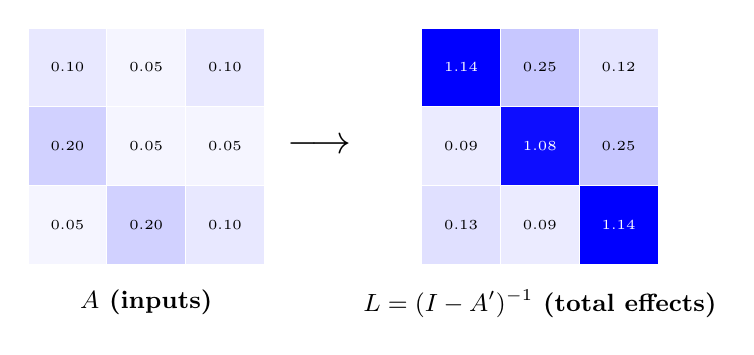
\begin{tikzpicture}[scale=1]
\def\s{1.0}
\foreach \i/\j/\v/\lab/\tc in {1/1/9/0.10/black,1/2/4/0.05/black,1/3/9/0.10/black,2/1/18/0.20/black,2/2/4/0.05/black,2/3/4/0.05/black,3/1/4/0.05/black,3/2/18/0.20/black,3/3/9/0.10/black} {
  \fill[blue!\v, draw=white, line width=0.3pt]
    ({(\j-1)*\s}, {(3-\i)*\s}) rectangle +(\s,\s);
  \node[font=\tiny, text=\tc] at ({(\j-0.5)*\s}, {(3-\i+0.5)*\s}) {\lab};
}
\node[below, font=\small\bfseries] at ({1.5*\s}, -0.2) {$A$ (inputs)};
\node[font=\Large] at (3.7, 1.5) {$\longrightarrow$};
\begin{scope}[xshift=5cm]
\foreach \i/\j/\v/\lab/\tc in {1/1/100/1.14/white,1/2/22/0.25/black,1/3/10/0.12/black,2/1/8/0.09/black,2/2/95/1.08/white,2/3/22/0.25/black,3/1/12/0.13/black,3/2/8/0.09/black,3/3/100/1.14/white} {
  \fill[blue!\v, draw=white, line width=0.3pt]
    ({(\j-1)*\s}, {(3-\i)*\s}) rectangle +(\s,\s);
  \node[font=\tiny, text=\tc] at ({(\j-0.5)*\s}, {(3-\i+0.5)*\s}) {\lab};
}
\node[below, font=\small\bfseries] at ({1.5*\s}, -0.2) {$L = (I-A')^{-1}$ (total effects)};
\end{scope}
\end{tikzpicture}
\end{center}
\vspace{-0.5em}
\small Both panels use one colour scale, from 0 (white) to 1.14 (the largest entry of $L$). The input matrix $A$ of Example~\ref{ch01:ex:IO} (left) is dim: weak direct dependencies. The Leontief inverse $L = (I-A')^{-1}$ (right; Example~\ref{ch01:ex:leontief_numbers}) is brighter --- indirect effects add to direct ones. Its diagonal is brightest because each unit of final demand requires at least one unit of own output. Bright off-diagonal cells mean demand propagates across sectors; dark ones (a block-diagonal $A$) mean it stays localized.
\end{vizpanel}


%% =====================================================================
\section{General Equilibrium: Markets Clear}
\label{ch01:sec:GE}
%% =====================================================================

\subsection{The Walrasian Equilibrium}

We now combine consumption and production. The economy has $N$ agents, $L$ goods, prices $p$, and an allocation $X$.

\begin{definition}[Walrasian Equilibrium]\label{ch01:def:walrasian}
A \textbf{Walrasian equilibrium} is a price vector $p^*$ and an allocation $X^*$ such that:
\begin{enumerate}
\item Every agent optimizes: $x_i^*$ solves~\eqref{ch01:eq:consumer} at prices $p^*$.
\item Markets clear: $\ones'X^* = \ones'\Omega$ (total demand equals total supply for each good).
\end{enumerate}
\end{definition}

The equilibrium $p^*$ is a \textit{fixed point}: it is the price at which the demands generated by $p^*$ are exactly consistent with $p^*$. Under standard conditions (continuous preferences, positive endowments), such a price exists --- this is the content of the Arrow-Debreu existence theorem, proved using Brouwer's fixed-point theorem.

We will not reproduce the proof here \citep[see][Chapter~17]{mascolell1995microeconomic}. The textbook proof is written for agents who interact only through $p$, but existence survives other channels: Debreu's \citeyearpar{debreu1952social} social-equilibrium theorem already covers consumption externalities. What externalities destroy is \textit{efficiency}, not existence (Chapter~2). Chapter~7 returns to existence for the bargaining equilibrium used in this book.


%% =====================================================================
\section{The Implicit Weight Matrix}
\label{ch01:sec:implicit_W}
%% =====================================================================

We are now ready for the chapter's punchline. 

\subsection{How Do Agents Interact in the Standard Model?}

Consider the economy we have developed: $N$ agents, each maximizing $U_i(x_i)$ subject to $p'x_i \leq w_i$, with market-clearing prices $p^*$. How does agent $i$ affect agent $j$?

The answer: only through $p^*$. Agent $i$'s demand for goods affects aggregate demand, which affects the equilibrium price, which affects $j$'s budget set and optimal choice. The interaction is:

\begin{enumerate}[label=(\alph*)]
\item \textbf{Anonymous}: the effect does not depend on who $i$ is --- only on $i$'s demand.
\item \textbf{Wealth-weighted}: in the aggregate, agent $i$'s demand counts in proportion to her expenditure. In the Cobb-Douglas economy, aggregate demand for good $\ell$ is $\sum_i w_i/(2p_\ell)$, so agent $i$'s weight is her \textbf{wealth share} $s_i = w_i/\sum_j w_j$. At the equilibrium of Section~\ref{ch01:sec:consumer}, $\mathbf{s} = (6.8, 5.8, 3.4)/16 = (0.425, 0.363, 0.213)$ --- not $(1/3, 1/3, 1/3)$.
\item \textbf{Indirect}: $i$ does not enter $j$'s utility function. The effect passes through the market.
\item \textbf{Price-taking}: no single agent's choice moves $p$ by a non-negligible amount; everyone takes the aggregate as given.
\end{enumerate}

These four properties describe a very specific pattern of interaction. We can write it as a matrix.

\subsection{Naming the Matrix}

\begin{definition}[The Market Interaction Matrix]\label{ch01:def:market_W}
Let $\mathbf{s}$ be the vector of wealth (expenditure) shares, $s_i = w_i/\sum_j w_j$. The \textbf{market interaction matrix} is
\begin{equation}\label{ch01:eq:W_mkt}
W^{\text{mkt}} = \ones\mathbf{s}'.
\end{equation}
Every row is the same vector $\mathbf{s}'$: each agent interacts with the market aggregate, in which agent $j$ carries weight $s_j$. Applied to any vector, $W^{\text{mkt}}\x = (\mathbf{s}'\x)\ones$ replaces every entry by the wealth-weighted mean.
\end{definition}

\begin{definition}[The Competitive Benchmark]\label{ch01:def:competitive_W}
With equal endowments, $\mathbf{s} = \frac{1}{N}\ones$ and the market interaction matrix becomes the \textbf{competitive benchmark}
\begin{equation}\label{ch01:eq:W_CE}
W^{CE} = \frac{1}{N}\ones\ones' = \frac{1}{N}\begin{pmatrix} 1 & 1 & \cdots & 1 \\ 1 & 1 & \cdots & 1 \\ \vdots & & \ddots & \vdots \\ 1 & 1 & \cdots & 1 \end{pmatrix}.
\end{equation}
Every entry is $1/N$: each agent affects every other agent equally.
\end{definition}

$W^{\text{mkt}}$ is what the Walrasian model implies; $W^{CE}$ is its equal-endowment special case, and the benchmark this book measures departures from. It has remarkable properties, which we now catalog.

\begin{proposition}[Properties of the Competitive Interaction Matrix]\label{ch01:prop:W_CE}
$W^{CE} = \frac{1}{N}\ones\ones'$ satisfies:
\begin{enumerate}
\item \textbf{Doubly stochastic}: every row sums to 1, and every column sums to 1. Nobody gives or receives more total influence than anyone else.
\item \textbf{Symmetric}: $W^{CE} = (W^{CE})'$. The effect of $i$ on $j$ equals the effect of $j$ on $i$.
\item \textbf{Rank 1}: all rows are identical. The matrix can be written as the outer product of two vectors: $W^{CE} = \frac{1}{N}\ones \cdot \ones'$. This means $W^{CE}$ contains \textit{no information about individual positions} --- every agent looks the same.
\item \textbf{Equal power}: its Perron vector (Section~\ref{ch01:sec:conventions}) is uniform, $\boldsymbol{\pi} = \frac{1}{N}\ones$.
\item \textbf{Unit spectral gap}: $W^{CE}$ has eigenvalue 1 (with eigenvector $\ones$) and eigenvalue 0 (with multiplicity $N-1$), so $\Gamma = 1 - |\lambda_2| = 1$. (See Appendix~\ref{ch01:app:spectral_radius} for eigenvalues.)
\end{enumerate}
Properties (3) and (5) are shared by every rank-one row-stochastic matrix, including $W^{\text{mkt}} = \ones\mathbf{s}'$ for any $\mathbf{s}$. What singles out $W^{CE}$ is (4): it is the only rank-one row-stochastic matrix with uniform $\boldsymbol{\pi}$.
\end{proposition}

\begin{proof}
(1) $\sum_j W^{CE}_{ij} = \sum_j 1/N = 1$. Similarly for column sums.

(2) $(W^{CE})' = (1/N \cdot \ones\ones')' = 1/N \cdot \ones\ones' = W^{CE}$.

(3) Every row is $(1/N, 1/N, \ldots, 1/N)$, so all rows are proportional (in fact, identical). Rank $= 1$.

(4) $\frac{1}{N}\ones'W^{CE} = \frac{1}{N^2}(\ones'\ones)\ones' = \frac{1}{N}\ones'$, so $\frac{1}{N}\ones$ is a stationary vector; it is the unique one because $W^{CE} > 0$ is irreducible (Perron--Frobenius, Chapter~6, Theorem~\ref{ch06:thm:PF}). Uniqueness of $W^{CE}$ among rank-one row-stochastic matrices with uniform $\boldsymbol{\pi}$: Section~\ref{ch01:sec:conventions}.

(5) $W^{CE}\ones = \frac{1}{N}\ones(\ones'\ones) = \frac{1}{N}\ones \cdot N = \ones$, so $\ones$ is an eigenvector with eigenvalue 1. For any $\x$ perpendicular to $\ones$ (i.e., $\ones'\x = 0$): $W^{CE}\x = \frac{1}{N}\ones(\ones'\x) = 0$. So eigenvalue 0 has multiplicity $N-1$.
\end{proof}

\begin{intuition}[What $W^{CE}$ does to a vector]
Apply $W^{CE}$ to any vector $\x$:
\begin{equation}
W^{CE}\x = \frac{1}{N}\ones(\ones'\x) = \bar{x} \cdot \ones,
\end{equation}
where $\bar{x} = \frac{1}{N}\sum_i x_i$ is the mean.

The competitive benchmark \textbf{replaces every entry with the mean}. It destroys all information about individual positions and keeps only the aggregate. The market matrix $W^{\text{mkt}}$ does the same with the wealth-weighted mean $\mathbf{s}'\x$: individual identities are washed out by the price mechanism, and only the aggregate (total demand, total supply) determines the outcome. Wealth, however, is not washed out.
\end{intuition}


\subsection{The Autarky Matrix}

The other extreme is no interaction at all:
\begin{equation}
W^A = I = \begin{pmatrix} 1 & 0 & \cdots & 0 \\ 0 & 1 & \cdots & 0 \\ \vdots & & \ddots & \vdots \\ 0 & 0 & \cdots & 1 \end{pmatrix}.
\end{equation}

Each agent interacts only with herself. No trade, no externalities, no social contact. Robinson Crusoe, $N$ times. As a weight matrix, $I$ is reducible: every probability vector is stationary, so power $\boldsymbol{\pi}$ is not defined, and $\Gamma = 0$.


\subsection{The Space of All Possible Structures}

Between $W = I$ (autarky) and $W^{\text{mkt}} = \ones\mathbf{s}'$ (anonymous competitive market) lies a vast space of possible interaction structures. Most real economies live somewhere in this space:

\begin{center}
\small
\begin{tabularx}{\textwidth}{lLLL}
\toprule
& \textbf{Autarky} & \textbf{General} $W$ & \textbf{Competitive} \\
& $W = I$ & & $W^{\text{mkt}} = \ones\mathbf{s}'$ \\
\midrule
Interaction & None & Structured & Anonymous \\
Power $\boldsymbol{\pi}$ & Undefined (reducible) & $\boldsymbol{\pi}(W)$, computed & $\mathbf{s}$ ($= \frac{1}{N}\ones$ if equal endowments) \\
Utility interdependence & None & $W^U \neq 0$ possible & $W^U = 0$ \\
Welfare theorems & Fail (no gains from trade) & FWT fails if $W^U \neq 0$ & Hold, for any $\mathbf{s}$ \\
\bottomrule
\end{tabularx}
\end{center}

\begin{keyinsight}
The program of this book is now visible. The benchmark competitive model lives at the right edge of this table. Its interaction is anonymous and rank one, $W^{\text{mkt}} = \ones\mathbf{s}'$, with no utility interdependence; with equal endowments it is $W^{CE}$. The First Welfare Theorem holds for \textit{any} wealth distribution $\mathbf{s}$; what it needs, in our language, is $W^U = 0$ together with complete markets and price-taking. The model does not assume equal power --- it assumes that power does not enter, because nobody bargains.

Structural economics replaces anonymous interaction with a general $W$: non-anonymous, possibly fragmented (slow integration, small $\Gamma$), and with a power distribution $\boldsymbol{\pi}$ that the network produces. Power becomes endogenous (Chapter~6). Preferences become endogenous to the network (Chapter~10). Externalities break efficiency (Chapter~2); unequal power is distributional, and the book asks how it is produced and changed. The question shifts from ``is the equilibrium efficient?'' to ``what is the structure, who does it benefit, and can it be changed?''

The standard model is not wrong. It is a special case. This book is the general case.
\end{keyinsight}

\begin{vizpanel}{$W^{CE}$ vs.\ the real world}
\begin{center}
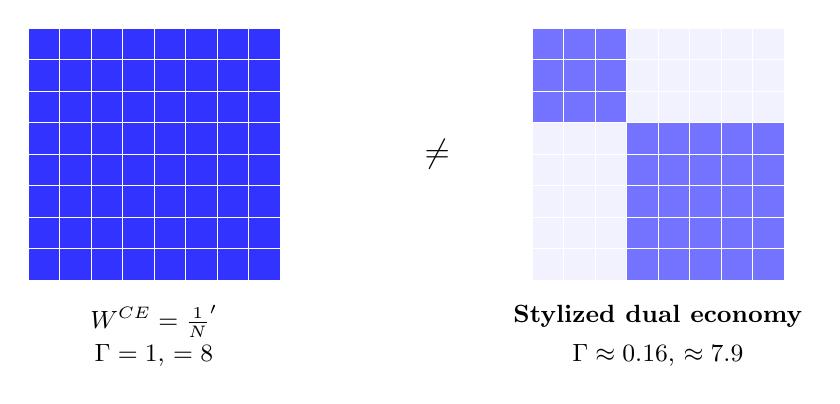
\begin{tikzpicture}[scale=1]
\def\N{8}
\def\s{0.4}
\foreach \i in {1,...,\N} {
  \foreach \j in {1,...,\N} {
    \fill[blue!80!white, draw=white, line width=0.15pt]
      ({(\j-1)*\s}, {(\N-\i)*\s}) rectangle +(\s,\s);
  }
}
\node[below, font=\small\bfseries] at ({4*\s}, -0.2) {$W^{CE} = \frac{1}{N}\ones\ones'$};
\node[below, font=\small] at ({4*\s}, -0.7) {$\Gamma = 1$, $\Neff = 8$};
\node[font=\large] at (5.2, 1.6) {$\neq$};
\begin{scope}[xshift=6.4cm]
\foreach \i in {1,...,\N} {
  \foreach \j in {1,...,\N} {
    \pgfmathparse{(\i<=3 && \j<=3) ? 70 : (\i>3 && \j>3) ? 55 : 5}
    \edef\bp{\pgfmathresult}
    \fill[blue!\bp, draw=white, line width=0.15pt]
      ({(\j-1)*\s}, {(\N-\i)*\s}) rectangle +(\s,\s);
  }
}
\node[below, font=\small\bfseries] at ({4*\s}, -0.2) {Stylized dual economy \illustrative};
\node[below, font=\small] at ({4*\s}, -0.7) {$\Gamma \approx 0.16$, $\Neff \approx 7.9$};
\end{scope}
\end{tikzpicture}
\end{center}
\vspace{-0.5em}
\small Left: the competitive benchmark (Prologue pattern~2, ``Market''). Right: a stylized dual economy (pattern~6, ``Dual Economy''; cell weights 70, 55 and 5, rows normalized), not an estimate for any country. Its two blocks are weakly coupled, so it integrates slowly ($\Gamma \approx 0.16$), yet power is almost uniform ($\Neff \approx 7.9$ of 8). Weak integration and power concentration are different properties (Section~\ref{ch01:sec:conventions}); the book studies both.
\end{vizpanel}


%% =====================================================================
\section{Conventions Used Throughout the Book}
\label{ch01:sec:conventions}
%% =====================================================================

The rest of the book uses the objects introduced above in a fixed way. This section states the conventions once; later chapters cite it rather than restating them.

\subsection{Matrices and Normalization}

\paragraph{Interaction matrices are row-stochastic.} An \textbf{interaction (weight) matrix} is a nonnegative $N \times N$ matrix $W$ with $W\ones = \ones$; $W_{ij}$ is the weight agent $i$ places on agent $j$. This covers the information network $W^I$, the utility network $W^U$, composites, and any generic $W$ whose Perron vector is read as power. A raw nonnegative matrix $K$ (counts, flows, overlaps) is turned into a weight matrix by row normalization, $W = D^{-1}K$ with $D = \text{diag}(K\ones)$; we say so whenever we do it.

\paragraph{Production uses two different objects.}
\begin{itemize}
\item The \textbf{technical-coefficient matrix} $A$ of Definition~\ref{ch01:def:IO}: $a_{ij}$ is the amount of good $j$ needed per unit of good $i$, so row $i$ is sector $i$'s recipe. The balance is $\y = A'\y + \mathbf{d}$ and the Leontief inverse is $L = (I - A')^{-1}$, which requires $\rho(A) < 1$. Output multipliers and backward/forward linkages are computed from $A$ (or a social-accounting coefficient matrix), never from a row-normalized matrix.
\item The \textbf{production weight matrix} $W^P := D^{-1}A$ with $D = \text{diag}(A\ones)$: row $i$ gives the input-cost shares of sector $i$. It is row-stochastic, and it is the input-share matrix of \citet{acemoglu2012network}. It is the object whose Perron vector and spectral gap we compute.
\end{itemize}
The reason for the separation: for \textit{any} row-stochastic $W$ and $0 \le \gamma < 1$, $(I - \gamma W)\ones = (1-\gamma)\ones$, hence $(I - \gamma W)^{-1}\ones = \frac{1}{1-\gamma}\ones$. All row-sum ``linkages'' of a row-normalized matrix coincide and carry no information.

\paragraph{Composites.} A composite $W = \sum_k \alpha_k W^k$ requires $\alpha_k \ge 0$, $\sum_k \alpha_k = 1$, and every layer $W^k$ row-stochastic on the \textit{same} node set. Layers defined on different node sets (sectors, media outlets, individuals) do not form a composite.

\subsection{Power: the Perron Vector}

\begin{definition}[Perron Vector]\label{ch01:def:perron}
For an irreducible row-stochastic $W$, the \textbf{Perron vector} $\boldsymbol{\pi}$ is the unique vector with $\boldsymbol{\pi}'W = \boldsymbol{\pi}'$, $\boldsymbol{\pi} > 0$ and $\sum_i \pi_i = 1$. (Existence and uniqueness: Perron--Frobenius, Chapter~6.)
\end{definition}

Each chapter states which of three readings of $\boldsymbol{\pi}$ is in force:
\begin{enumerate}
\item \textbf{Information (DeGroot).} If beliefs update as $\mathbf{b}^{(t+1)} = W\mathbf{b}^{(t)}$, the consensus is $b^* = \boldsymbol{\pi}'\mathbf{b}^{(0)}$: $\pi_j$ is exactly agent $j$'s weight in the long-run consensus. If $W$ is also aperiodic, $W^t \to \ones\boldsymbol{\pi}'$ and the beliefs converge to it.
\item \textbf{Production.} $\boldsymbol{\pi}' = \lim_{\gamma \to 1} \frac{1-\gamma}{N}\ones'(I - \gamma W^P)^{-1}$, the limit of the normalized influence vector. For $\gamma < 1$, the influence vector of \citet{acemoglu2012network}, $\frac{\alpha}{N}\ones'(I - (1-\alpha)W^P)^{-1}$, is a Katz/Leontief object, not the Perron vector.
\item \textbf{Bargaining.} Using $\boldsymbol{\pi}$ as the Nash weights $\boldsymbol{\lambda}$ of Definition~\ref{ch01:def:bargaining_power} is a \textbf{modelling assumption}, not a result. In strategic models of bargaining on networks \citep{manea2011bargaining,abreu2012bargaining,abreu2012markov}, payoffs are generally \textit{not} eigenvector centralities.
\end{enumerate}
For the market matrix, $\boldsymbol{\pi}(W^{\text{mkt}}) = \mathbf{s}$: since $\mathbf{s}'\ones\mathbf{s}' = \mathbf{s}'$, wealth shares are the market's ``power'' vector.

\paragraph{Measuring concentration.} Unequal power means a concentrated $\boldsymbol{\pi}$. We measure it by:
\begin{itemize}
\item the \textbf{effective number of agents} $\Neff = 1/\sum_i \pi_i^2 \in [1, N]$;
\item the \textbf{variance of power} $\Var(\pi) = \frac{1}{N}\sum_i (\pi_i - \frac{1}{N})^2 = \frac{1}{N}\bigl(\frac{1}{\Neff} - \frac{1}{N}\bigr)$, which uses $\sum_i(\pi_i - \frac1N)^2 = \sum_i\pi_i^2 - \frac{1}{N}$. Its maximum is $(N-1)/N^2$, attained at $\boldsymbol{\pi} = e_1$: $0.1875$ for $N = 4$, $0.0475$ for $N = 20$;
\item the \textbf{power distance} $d_\pi = \frac{1}{2}\|\boldsymbol{\pi} - \frac{1}{N}\ones\|_1 \in [0, 1 - \frac1N]$, and the power Gini.
\end{itemize}
In the Cobb-Douglas equilibrium of Section~\ref{ch01:sec:consumer}, $\Neff(\mathbf{s}) = 2.80$ of $3$.

\begin{proposition}[When Power Is Uniform]\label{ch01:prop:pi_uniform}
For an irreducible row-stochastic $W$, $\boldsymbol{\pi} = \frac{1}{N}\ones$ if and only if $W$ is doubly stochastic.
\end{proposition}
\begin{proof}
If $\ones'W = \ones'$, then $\frac{1}{N}\ones'$ is a stationary probability vector, and by uniqueness of the stationary vector of an irreducible stochastic matrix (Perron--Frobenius; \citealt[Thm.~8.4.4]{horn2012matrix}) it equals $\boldsymbol{\pi}'$. Conversely, $\frac{1}{N}\ones'W = \frac{1}{N}\ones'$ says every column sums to one.
\end{proof}
For a nonnegative $W$ that is \textit{not} row-stochastic, the condition is ``all column sums equal'', which is why we avoid non-stochastic $W$ when $\boldsymbol{\pi}$ is read as power.

\subsection{The Spectral Gap Measures Integration}

\begin{definition}[Spectral Gap]\label{ch01:def:gap}
For a row-stochastic $W$ with eigenvalues ordered $1 = |\lambda_1| \ge |\lambda_2| \ge \cdots$, the \textbf{spectral gap} is $\Gap(W) = 1 - |\lambda_2(W)|$.
\end{definition}

$\Gap$ measures \textbf{integration}: deviations from consensus (or from the stationary distribution) decay like $|\lambda_2|^t$, with half-life $\ln 2/(-\ln|\lambda_2|)$. $\Gap = 0$ when $W$ is reducible (several unit eigenvalues, as for $W = I$) \textit{or} periodic (an eigenvalue of modulus one other than 1, as for a bipartite star or an even ring without self-loops); the lazy version $\frac{1}{2}(I + W)$ removes periodicity. For reversible $W$ with conductance $\Phi_c$, Cheeger's inequality $\Phi_c^2/2 \le 1 - \lambda_2 \le 2\Phi_c$ \citep[Thm.~13.14]{levin2009markov} says that weak cross-block coupling implies a small gap. The converse fails: a small gap can come from periodicity rather than fragmentation.

\textbf{$\Gap$ does not measure power.} For every $\boldsymbol{\pi}$ in the open simplex and every $\gamma \in (0, 1]$, the matrix $W = \gamma\,\ones\boldsymbol{\pi}' + (1-\gamma)I$ is irreducible, aperiodic and row-stochastic, with $\boldsymbol{\pi}(W) = \boldsymbol{\pi}$ (because $\boldsymbol{\pi}'W = \gamma\boldsymbol{\pi}' + (1-\gamma)\boldsymbol{\pi}'$) and spectrum $\{1, 1-\gamma, \ldots, 1-\gamma\}$, so $\Gap(W) = \gamma$. Any degree of concentration is compatible with any gap (Chapter~6, Proposition~\ref{ch06:prop:gap-power-independent}). With $N = 10$ and $\pi_1 = 0.91$, $\Neff = 1.21$ for every $\gamma$, while $\Gap$ ranges over $(0, 1]$. The stylized dual economy in the visualization above makes the opposite point: small $\Gap$ with almost uniform power.

\subsection{Distance from the Benchmark}

We write $\Delta(W) := W - W^{CE}$ for the departure from the benchmark and summarize it by \textbf{two} coordinates, which the example above shows to be independent: the power distance $d_\pi$ (or $\Neff/N$) and the integration deficit $1 - \Gap$.

Two facts about the benchmark. Every rank-one row-stochastic matrix has the form $\ones\boldsymbol{\pi}'$ (if $W = \mathbf{u}\mathbf{v}'$ and $W\ones = \ones$, then $\mathbf{u} \propto \ones$), and its Perron vector is $\boldsymbol{\pi}$. Hence $W^{CE}$ is the \textit{unique} rank-one row-stochastic matrix with uniform power. No scalar norm of $\Delta(W)$ determines welfare: outcomes depend on $W$ \textit{and} on primitives (curvature, endowments, the game being played) that are not functions of $\Delta(W)$.

\subsection{The Competitive Benchmark and the Welfare Theorems}

The statement used throughout the book is:
\begin{itemize}
\item Walrasian price formation is anonymous. Aggregate demand weights agents by wealth shares $\mathbf{s}$, so the implied interaction matrix is $W^{\text{mkt}} = \ones\mathbf{s}'$: rank one, $\Gap = 1$, $\boldsymbol{\pi} = \mathbf{s}$. The benchmark $W^{CE} = \frac{1}{N}\ones\ones'$ is the equal-endowment special case.
\item The First Welfare Theorem holds for \textit{any} $\mathbf{s}$. It requires local nonsatiation, complete markets, price-taking and no externalities --- in this book's language, $W^U = 0$.
\item Utility interdependence ($W^U \neq 0$) and missing markets break efficiency. Non-anonymous interaction with unequal $\boldsymbol{\pi}$ is \textbf{distributional}: weighted Nash bargaining is Pareto efficient (Proposition~\ref{ch01:prop:nash_division}), and the associated loss is a utilitarian loss, not a Pareto inefficiency.
\item Autarky ($W = I$) is not a case in which the welfare theorems ``trivially hold'': the gains from trade go unrealized.
\end{itemize}
The textbook benchmark is thus anonymous interaction with no externalities --- in its equal-endowment form, $W = W^{CE}$. Structural economics studies non-anonymous $W$ (its structure: blocks, integration $\Gap$) and the distribution of power $\boldsymbol{\pi}$, and how both are produced and changed.

\subsection{The Allocation Rule and the Calibration of Utility}

\begin{proposition}[The Allocation Rule]\label{ch01:prop:allocation_rule}
In the transferable-utility bargaining problem of Definition~\ref{ch01:def:nash}, let the weights be $\boldsymbol{\lambda} = \boldsymbol{\pi}$, the Perron vector of an irreducible row-stochastic $W$ (so $\pi_i > 0$), and let all disagreement payoffs be equal, $d_i = \bar d$. Define the bargaining surplus $\Phi := \Omega - N\bar d$ and assume $\Phi > 0$. Then
\begin{equation}\label{ch01:eq:allocation_rule}
x_i = \frac{\Omega}{N} + \Bigl(\pi_i - \frac{1}{N}\Bigr)\Phi.
\end{equation}
If utility is $U(x) = x - \frac{\kappa}{2}x^2$, the utilitarian loss relative to equal division is exactly
\begin{equation}\label{ch01:eq:L_power}
L_{\text{power}} := \sum_i \Bigl[U\bigl(\tfrac{\Omega}{N}\bigr) - U(x_i)\Bigr] = \frac{\kappa N}{2}\,\Phi^2\,\Var(\pi).
\end{equation}
\end{proposition}
\begin{proof}
The hypotheses of Proposition~\ref{ch01:prop:nash_division} hold ($\pi_i > 0$, $\Omega - \sum_j d_j = \Phi > 0$), so by~\eqref{ch01:eq:nash_division}, $x_i = \bar d + \pi_i\Phi = \frac{\Omega}{N} + (\pi_i - \frac1N)\Phi$, since $\bar d = \frac{\Omega}{N} - \frac{\Phi}{N}$. Write $m = \Omega/N$ and $z_i = x_i - m$, so $\sum_i z_i = 0$. Because $U$ is quadratic, $U(m + z_i) = U(m) + U'(m)z_i - \frac{\kappa}{2}z_i^2$ exactly. Summing, the linear terms cancel and $L_{\text{power}} = \frac{\kappa}{2}\sum_i z_i^2 = \frac{\kappa}{2}\Phi^2\sum_i(\pi_i - \frac1N)^2 = \frac{\kappa N}{2}\Phi^2\Var(\pi)$.
\end{proof}

Chapter~7 derives the same rule in the network setting (Proposition~\ref{ch07:prop:allocation-rule}). Two cautions. First, $\Phi$ is the \textit{surplus over disagreement}, not a curvature parameter. In a one-good exchange economy with endowments as the disagreement point there is nothing to bargain over and $\Phi = 0$. Second, every allocation used in an example must satisfy $\kappa x_i < 1$, so that utility is increasing. Past the satiation point $1/\kappa$, ``getting more'' makes an agent worse off and the welfare comparisons become meaningless. For example, with $\Omega = 3$, $\bar d = 0.3$ (so $\Phi = 2.1$), $\boldsymbol{\pi} = (0.6, 0.2, 0.2)$ and $\kappa = 0.5$: $\x = (1.56, 0.72, 0.72)$, $\Var(\pi) = 0.0356$, and $L_{\text{power}} = 0.75 \times 4.41 \times 0.0356 = 0.118$.


%% =====================================================================
\section{Summary}
\label{ch01:sec:summary}
%% =====================================================================

This chapter established five results, all of them standard economics expressed in matrix notation:

\begin{enumerate}
\item The \textbf{allocation matrix} $X$ organizes who gets what. Read by rows: individual bundles. Read by columns: distribution of each good. The rank of $X$ measures structural differentiation.

\item The \textbf{consumer's problem} determines each row of $X$ independently under the standard model. Agent $i$'s utility depends only on $x_i$. This is a structural assumption: the weight agent $i$ places on agent $j$'s consumption is zero.

\item The \textbf{welfare loss from inequality} in the one-good economy is $L = \frac{\kappa N}{2}\text{Var}(\omega_i)$. With Nash bargaining over a joint surplus, $x_i = d_i + \lambda_i(\Omega - \sum_j d_j)$: the allocation depends on who has power, not just on who has outside options. The resulting loss is distributional, not a Pareto inefficiency.

\item The \textbf{Leontief inverse} $(I - A')^{-1}$ is the first structural matrix in standard economics. It encodes all direct and indirect inter-sectoral dependencies. Its properties (column sums, spectral radius) characterize the production structure.

\item The \textbf{implicit interaction matrix} of the competitive model is $W^{\text{mkt}} = \ones\mathbf{s}'$: anonymous, rank one, $\Gap = 1$, with power equal to wealth shares; its equal-endowment case is the benchmark $W^{CE} = \frac{1}{N}\ones\ones'$. The First Welfare Theorem holds for any $\mathbf{s}$ provided $W^U = 0$. Power concentration ($\Neff$, $\Var(\pi)$) and integration ($\Gap$) are independent coordinates of a general $W$ (Section~\ref{ch01:sec:conventions}).
\end{enumerate}

No new economics was introduced. But the notation reveals an object --- the weight matrix $W$ --- that was always present but never named. The next chapters will show what changes when $W$ is not anonymous.


%% =====================================================================
\section{Exercises}
\label{ch01:sec:exercises}
%% =====================================================================

\begin{enumerate}[label=\textbf{1.\arabic*}, leftmargin=3em]

\item \textbf{Reading the allocation matrix.} For $N = 4$ agents and $L = 3$ goods (Food, Clothing, Housing), the allocation matrix is:
\begin{equation}
X = \begin{pmatrix} 5 & 3 & 1 \\ 2 & 4 & 2 \\ 1 & 1 & 5 \\ 4 & 2 & 2 \end{pmatrix}.
\end{equation}
\begin{enumerate}
\item What is agent 3's consumption bundle? What is agent 3 likely ``good at'' (what might she produce)?
\item What is the total consumption of Housing? Which agent consumes the most Housing?
\item Is this allocation feasible if total endowments are $\ones'\Omega = (12, 10, 10)$?
\item Compute the rank of $X$. Is this a ``structurally differentiated'' economy in the sense discussed above?
\end{enumerate}

\item \textbf{Cobb-Douglas equilibrium.} Three agents with $U_i = x_{i1}^{1/3}x_{i2}^{2/3}$ and endowments $\omega_1 = (4, 1)'$, $\omega_2 = (1, 3)'$, $\omega_3 = (3, 2)'$.
\begin{enumerate}
\item Derive the Marshallian demand functions.
\item Find the equilibrium price $p_2^*$ (normalize $p_1 = 1$) by solving the market-clearing condition.
\item Compute the equilibrium allocation $X^*$ and verify feasibility.
\end{enumerate}

\item \textbf{Welfare loss computation.} For $N = 5$, $\kappa = 0.1$, $\Omega = 5$ (check that $\kappa\omega_i < 1$ in every case):
\begin{enumerate}
\item Compute $L$ for $\boldsymbol{\omega} = (1, 1, 1, 1, 1)$. (Answer: 0.)
\item Compute $L$ for $\boldsymbol{\omega} = (3, 1, 0.5, 0.25, 0.25)$.
\item Compute $L$ for $\boldsymbol{\omega} = (5, 0, 0, 0, 0)$ (one person has everything).
\item Plot $L$ as a function of the Gini coefficient of $\boldsymbol{\omega}$.
\end{enumerate}

\item \textbf{Bargaining with different power.} Two agents ($N = 2$, $\kappa = 0.5$) produce $\Omega = 2$ together; their disagreement payoffs are $\mathbf{d} = (0.6, 0.2)$. Use Proposition~\ref{ch01:prop:nash_division}.
\begin{enumerate}
\item Find the first-best (utilitarian) allocation and welfare.
\item Find the bargaining allocation for $\boldsymbol{\lambda} = (0.5, 0.5)$ (equal power). Compare to the first-best.
\item Find the bargaining allocation for $\boldsymbol{\lambda} = (0.8, 0.2)$ (asymmetric power). Who benefits?
\item For what $\boldsymbol{\lambda}$ does the bargaining allocation equal the first-best?
\end{enumerate}

\item \textbf{The cascade in action.} For the input-output matrix:
\begin{equation}
A = \begin{pmatrix} 0.2 & 0.1 \\ 0.3 & 0.1 \end{pmatrix}.
\end{equation}
\begin{enumerate}
\item Compute the first five terms of the Neumann series: $I$, $A'$, $(A')^2$, $(A')^3$, $(A')^4$. (Use a calculator or Python.)
\item Sum them: $\sum_{k=0}^4 (A')^k$. Compare with the exact $(I - A')^{-1}$. How close are they?
\item What is the spectral radius $\rho(A)$? (See Appendix~\ref{ch01:app:spectral_radius}.) Verify $\rho(A) < 1$.
\item Compute output multipliers (column sums of $(I - A')^{-1}$). Which sector has stronger backward linkages?
\end{enumerate}

\item \textbf{Properties of $W^{CE}$.}
\begin{enumerate}
\item Show that $W^{CE}$ is idempotent: $(W^{CE})^2 = W^{CE}$. (Hint: compute $\frac{1}{N}\ones\ones' \cdot \frac{1}{N}\ones\ones'$.)
\item Show that for any vector $\x$, $W^{CE}\x = \bar{x}\ones$. Interpret: the competitive market replaces individual variation with the average.
\item Prove: $W^{CE}$ has eigenvalue 1 with eigenvector $\ones$, and eigenvalue 0 with multiplicity $N-1$. Find the eigenvectors for eigenvalue 0 when $N = 3$.
\item For $N = 3$, consider the matrix $W = \frac{1}{3}\begin{pmatrix} 1 & 1 & 1 \\ 2 & 0.5 & 0.5 \\ 0 & 1.5 & 1.5 \end{pmatrix}$. Is this doubly stochastic? Compute $W\x$ for $\x = (3, 6, 9)'$ and compare with $W^{CE}\x$. What is different?
\end{enumerate}

\item \textbf{Bolivia's input-output table} (data exercise). Download the Bolivian input-output or supply-use tables from INE (Bolivia is not a separate economy in the OECD ICIO tables; multi-region alternatives that include it are Eora and CEPAL's regional input-output matrices). Aggregate to 5--10 sectors.
\begin{enumerate}
\item Construct $A$ in this book's convention: $a_{ij}$ = purchases by sector $i$ from sector $j$ divided by sector $i$'s gross output. (Published tables usually record sales from row $i$ to column $j$ and divide each \textit{column} by gross output; that matrix is $A'$ in our notation.)
\item Compute the Leontief inverse $(I - A')^{-1}$.
\item Compute output multipliers for: Mining/Gas, Agriculture, Manufacturing, Services.
\item Which sector has the highest multiplier? Lowest? Relate to Pinto's structural heterogeneity: is Bolivia's economy ``structurally connected'' or ``block-diagonal''?
\item \textit{Challenge}: Is the gas sector connected to the rest of the economy, or is it an enclave?
\end{enumerate}

\item \textbf{From story to matrix.} Do\~{n}a Mar\'{i}a sells api morado on Calle Comercio in La Paz. To produce api, she buys corn from a wholesaler in El Alto, sugar from a shop on Calle Max Paredes, cinnamon from a market distributor, and charcoal from a supplier in the altiplano. The wholesaler buys from farmers in the Yungas.
\begin{enumerate}
\item Define 5 agents: Mar\'{i}a, Wholesaler, Sugar Shop, Cinnamon Distributor, Charcoal Supplier. Draw the directed dependency graph.
\item Write the $5 \times 5$ adjacency matrix $A$ ($A_{ij} = 1$ if agent $i$ uses agent $j$'s output as input, 0 otherwise).
\item Is $A$ symmetric? What does the asymmetry mean economically?
\item Suppose the Wholesaler disappears. Set row and column 2 of $A$ to zero. Which other agents are directly affected? Which are indirectly affected (via the Leontief cascade)?
\item Compare this adjacency matrix to $W^{CE}$ for $N = 5$. What structural information does $A$ contain that $W^{CE}$ destroys?
\end{enumerate}

\item \textbf{From sectors to countries.} Suppose the ``agents'' in the Leontief system are 3 countries:
\begin{equation}
A = \begin{pmatrix} 0.05 & 0.30 & 0.30 \\ 0.01 & 0.05 & 0.05 \\ 0.01 & 0.05 & 0.05 \end{pmatrix}.
\end{equation}
Column 1 shows who needs Country 1's output: $0.05, 0.01, 0.01$ --- it is barely used by others. Row 1 shows that Country 1 needs a lot from Countries 2 and 3 ($0.30$ each).
\begin{enumerate}
\item Compute the output multipliers (column sums of $(I - A')^{-1}$). Which country has the strongest backward linkages?
\item If final demand rises by 1 unit in Country 2 only, how much total output is generated in each country?
\item In Prebisch's account the periphery exports primary goods to the center and imports manufactures \textit{from} it. Does this $A$ have that pattern, or its reverse? Modify $A$ so that Countries 2 and 3 depend on Country 1's output, and recompute (a).
\item Argue informally that the center-periphery structure is a property of the asymmetry of $A$.
\end{enumerate}
\end{enumerate}


%% =====================================================================
\newpage
\section*{Mathematical Appendices}
\addcontentsline{toc}{section}{Mathematical Appendices}
%% =====================================================================


%% =====================================================================
\subsection*{Appendix 1A: Matrices as Economic Objects}
\addcontentsline{toc}{subsection}{Appendix 1A: Matrices as Economic Objects}
\label{ch01:app:matrices}
%% =====================================================================

This appendix covers the matrix concepts used in Chapter~1, starting from scratch.

\paragraph{What is a matrix?} A matrix is a rectangular table of numbers. An $N \times L$ matrix has $N$ rows and $L$ columns. In this book, matrices represent \textit{relationships}: the entry in row $i$, column $j$ describes the relationship between agent (or sector) $i$ and agent (or sector) $j$.

\begin{center}
\begin{tabular}{ll}
\toprule
\textbf{Matrix} & \textbf{What it describes} \\
\midrule
Allocation $X$ ($N \times L$) & How much of each good each person consumes \\
Endowment $\Omega$ ($N \times L$) & How much of each good each person starts with \\
Input-output $A$ ($N \times N$) & How much of each sector's output each sector needs \\
Interaction $W$ ($N \times N$) & How much each agent affects each other agent \\
\bottomrule
\end{tabular}
\end{center}

\paragraph{Special vectors.} Two vectors appear constantly:
\begin{itemize}
\item $\ones = (1, 1, \ldots, 1)'$: the vector of all ones. $\ones'x = \sum_i x_i$ sums the entries of $x$.
\item $e_k$: the $k$-th standard basis vector (1 in position $k$, 0 elsewhere). $e_k'x = x_k$ picks out the $k$-th entry.
\end{itemize}

\paragraph{Matrix multiplication as ``flow through a system.''} If $A$ is $N \times N$ and $\x$ is $N \times 1$, then $A\x$ is $N \times 1$ with $(A\x)_i = \sum_j a_{ij}x_j$. Think of $x_j$ as the ``amount of stuff at node $j$'' and $a_{ij}$ as ``how much of node $j$'s stuff flows to node $i$.'' The product $A\x$ is the result of flowing everything through the system once.

Flow through twice: $A(A\x) = A^2\x$. Flow $k$ times: $A^k\x$. The Leontief inverse $(I - A)^{-1} = I + A + A^2 + \cdots$ sums the result of flowing through all possible numbers of times.

\paragraph{The outer product $\ones\ones'$.} This is an $N \times N$ matrix of all ones:
\begin{equation}
\ones\ones' = \begin{pmatrix} 1 \\ 1 \\ \vdots \\ 1 \end{pmatrix} \begin{pmatrix} 1 & 1 & \cdots & 1 \end{pmatrix} = \begin{pmatrix} 1 & 1 & \cdots & 1 \\ 1 & 1 & \cdots & 1 \\ \vdots & & \ddots & \vdots \\ 1 & 1 & \cdots & 1 \end{pmatrix}.
\end{equation}

Dividing by $N$ gives $W^{CE} = \frac{1}{N}\ones\ones'$, where every entry is $1/N$. This matrix has a beautiful property: $W^{CE}\x = \bar{x}\ones$ --- it replaces every entry of $\x$ with the mean. It is the mathematical representation of ``anonymous, symmetric interaction.''

\paragraph{The identity matrix $I$.} The $N \times N$ identity matrix has 1 on the diagonal and 0 elsewhere. $I\x = \x$ for any $\x$: it does nothing. It represents ``no interaction'' --- each agent affects only herself.

\paragraph{Row sums and column sums.} For an $N \times N$ matrix $M$:
\begin{itemize}
\item Row sums: $M\ones$ is an $N \times 1$ vector whose $i$-th entry is $\sum_j m_{ij}$ (total outflow from $i$).
\item Column sums: $\ones'M$ is a $1 \times N$ vector whose $j$-th entry is $\sum_i m_{ij}$ (total inflow to $j$).
\end{itemize}

A matrix is \textbf{row-stochastic} if all row sums equal 1: $M\ones = \ones$. It is \textbf{column-stochastic} if all column sums equal 1: $\ones'M = \ones'$. It is \textbf{doubly stochastic} if both. The competitive interaction matrix $W^{CE}$ is doubly stochastic.


%% =====================================================================
\subsection*{Appendix 1B: Eigenvalues and the Spectral Radius}
\addcontentsline{toc}{subsection}{Appendix 1B: Eigenvalues and the Spectral Radius}
\label{ch01:app:spectral_radius}
%% =====================================================================

\paragraph{The key idea.} An eigenvalue is a number that tells you how a matrix \textit{stretches} things. If $A\mathbf{v} = \lambda\mathbf{v}$ for some nonzero vector $\mathbf{v}$, then $\lambda$ is an eigenvalue and $\mathbf{v}$ is the corresponding eigenvector. Applying $A$ to $\mathbf{v}$ just rescales it by $\lambda$ --- the direction stays the same, only the magnitude changes.

\paragraph{Why economists care.} Eigenvalues tell you whether a system explodes, converges, or oscillates:
\begin{itemize}
\item $|\lambda| < 1$: applying $A$ repeatedly shrinks the component along $\mathbf{v}$. The system converges.
\item $|\lambda| = 1$: the component stays the same. Steady state.
\item $|\lambda| > 1$: the component grows without bound. Explosion.
\end{itemize}

\paragraph{The spectral radius.} The \textbf{spectral radius} of $A$ is $\rho(A) = \max_i |\lambda_i|$ --- the largest eigenvalue in magnitude. It determines the long-run behavior of the system:
\begin{itemize}
\item $\rho(A) < 1$: $A^k \to 0$ as $k \to \infty$. The cascade of indirect effects dies out. The Leontief inverse exists.
\item $\rho(A) = 1$: the system is on the boundary. Convergence is borderline.
\item $\rho(A) > 1$: $A^k$ explodes. The system requires more inputs than it produces. The economy is ``unproductive.''
\end{itemize}

For the input-output matrix, $\rho(A) < 1$ means the economy is productive: it produces more output than it uses as input.

\paragraph{Computing eigenvalues.} For a $2 \times 2$ matrix $A = \begin{pmatrix} a & b \\ c & d \end{pmatrix}$, the eigenvalues solve $\det(A - \lambda I) = 0$:
\begin{equation}
\lambda^2 - (a + d)\lambda + (ad - bc) = 0.
\end{equation}
The solutions are $\lambda = \frac{(a+d) \pm \sqrt{(a+d)^2 - 4(ad-bc)}}{2}$. For larger matrices, use numerical software.

\paragraph{Example.} For $A = \begin{pmatrix} 0.2 & 0.1 \\ 0.3 & 0.1 \end{pmatrix}$ (from Exercise~1.5): trace $= 0.3$, determinant $= 0.02 - 0.03 = -0.01$. Eigenvalues: $\lambda = \frac{0.3 \pm \sqrt{0.09 + 0.04}}{2} = \frac{0.3 \pm 0.36}{2}$. So $\lambda_1 = 0.33$ and $\lambda_2 = -0.03$. Spectral radius: $\rho(A) = 0.33 < 1$. The economy is productive.

\paragraph{The spectral gap.} For a row-stochastic $W$ the largest eigenvalue is $\lambda_1 = 1$, and the \textbf{spectral gap} is $\Gamma = 1 - |\lambda_2|$, where $\lambda_2$ is the eigenvalue of second-largest modulus (Definition~\ref{ch01:def:gap}). The spectral gap measures \textit{integration} --- how fast the system forgets its starting point:
\begin{itemize}
\item Large $\Gamma$: deviations from the long-run state die out quickly (like $|\lambda_2|^t$). Every rank-one matrix $\ones\boldsymbol{\pi}'$, including $W^{CE}$, has $\Gamma = 1$.
\item Small $\Gamma$: slow convergence. This happens when the network is split into weakly coupled blocks, or when it is periodic (a bipartite star or an even ring without self-loops has $\Gamma = 0$).
\end{itemize}

The spectral gap says nothing about how concentrated power is: Section~\ref{ch01:sec:conventions} shows that every $\boldsymbol{\pi}$ is compatible with every $\Gamma$. Chapter~6 develops these connections formally. For now: eigenvalues measure how a system amplifies or dampens, and the spectral gap measures how fast it integrates.


%% =====================================================================
\subsection*{Appendix 1C: The Neumann Series}
\addcontentsline{toc}{subsection}{Appendix 1C: The Neumann Series}
\label{ch01:app:neumann}
%% =====================================================================

\paragraph{Start with scalars.} You know the geometric series: if $|r| < 1$, then
\begin{equation}
1 + r + r^2 + r^3 + \cdots = \frac{1}{1 - r}.
\end{equation}

Rearranging: $(1 - r)(1 + r + r^2 + \cdots) = 1$, so $1 + r + r^2 + \cdots$ is the \textit{inverse} of $(1 - r)$.

\paragraph{Now matrices.} Replace the scalar $r$ with a matrix $A$ and the number 1 with the identity matrix $I$:
\begin{equation}\label{ch01:eq:neumann_app}
I + A + A^2 + A^3 + \cdots = (I - A)^{-1},
\end{equation}
provided the series converges. The condition for convergence is $\rho(A) < 1$ (the spectral radius is less than 1) --- the matrix analog of $|r| < 1$.

\paragraph{Why it converges.} The entries of $A^k$ are \textit{not} bounded by $\rho(A)^k$ in general (for $A = \begin{pmatrix} 0.5 & 0.9 \\ 0 & 0.5\end{pmatrix}$, $\rho = 0.5$ but $a_{12} = 0.9$). What is true is Gelfand's formula, $\|A^k\|^{1/k} \to \rho(A)$: for any $\varepsilon > 0$ there is a constant $C$ with $\|A^k\| \le C(\rho(A) + \varepsilon)^k$. Since $\rho(A) < 1$, choose $\varepsilon$ with $\rho(A) + \varepsilon < 1$; the powers decay geometrically and $A^k \to 0$ as $k \to \infty$. The partial sums $\sum_{k=0}^K A^k$ converge to a finite matrix, which is $(I - A)^{-1}$.

\paragraph{Verification.} Multiply a partial sum by $(I - A)$:
\begin{align}
(I - A)(I + A + \cdots + A^K) &= (I + A + \cdots + A^K) - (A + A^2 + \cdots + A^{K+1}) \\
&= I - A^{K+1}.
\end{align}
The sum telescopes. Since $A^{K+1} \to 0$, letting $K \to \infty$ gives $(I - A)\sum_{k=0}^\infty A^k = I$ (and likewise with the factors in the other order). This confirms that $\sum_{k=0}^\infty A^k$ is indeed the inverse of $(I - A)$.

\paragraph{Economic interpretation.} In the Leontief system:
\begin{itemize}
\item $I$: direct demand (round 0). Each unit of final demand requires one unit of direct output.
\item $A'$: first-round indirect demand. Producing the direct output requires $A'$ units of intermediate inputs.
\item $(A')^2$: second-round indirect demand. Producing the first-round inputs requires further inputs.
\item $(A')^k$: $k$-th round. The cascade continues.
\item $(I - A')^{-1}$: the total of all rounds. The complete direct + indirect requirement.
\end{itemize}

\paragraph{A numerical example.} For $A' = \begin{pmatrix} 0.2 & 0.3 \\ 0.1 & 0.1 \end{pmatrix}$:

\begin{center}
\begin{tabular}{l c c c c}
\toprule
& $(1,1)$ & $(1,2)$ & $(2,1)$ & $(2,2)$ \\
\midrule
$I$ & 1.000 & 0.000 & 0.000 & 1.000 \\
$I + A'$ & 1.200 & 0.300 & 0.100 & 1.100 \\
$I + A' + (A')^2$ & 1.270 & 0.390 & 0.130 & 1.140 \\
$I + A' + \cdots + (A')^3$ & 1.293 & 0.420 & 0.140 & 1.153 \\
$I + A' + \cdots + (A')^4$ & 1.301 & 0.430 & 0.143 & 1.157 \\
$(I - A')^{-1}$ (exact) & 1.304 & 0.435 & 0.145 & 1.159 \\
\bottomrule
\end{tabular}
\end{center}

By round 4, every entry of the partial sum is within about 1.1\% of the exact inverse. The cascade converges fast when $\rho(A)$ is small.


%% =====================================================================
\subsection*{Structuralist Case Study: Prebisch's 1949 Manifesto and the Weight Matrix}
\addcontentsline{toc}{subsection}{Structuralist Case Study: Prebisch (1949)}
%% =====================================================================

In 1949, Ra\'{u}l Prebisch --- an Argentine economist who had served as head of his country's central bank --- published what Albert Hirschman later called the ``Latin American Manifesto'': \textit{El desarrollo econ\'{o}mico de la Am\'{e}rica Latina y algunos de sus principales problemas}. The essay served as the introduction to CEPAL's first \textit{Estudio econ\'{o}mico de Am\'{e}rica Latina} and laid the intellectual foundation for half a century of structuralist economics.

Prebisch's argument has three steps, each of which corresponds to a property of the weight matrix developed in this chapter.

\textbf{Step 1: The global economy has a structure.} Prebisch rejected the presumption that the gains from trade and technical progress are spread evenly across trading partners. He argued that the world economy is divided into an industrialized ``center'' and a primary-commodity-exporting ``periphery,'' connected by trade linkages that are fundamentally \textit{asymmetric}: the periphery exports raw materials with low value-added and imports manufactures with high value-added. In the notation of this chapter, the hypothesis is that the global input-output matrix $A_{\text{global}}$ has a core-periphery topology: the center's column sums in the Leontief inverse $(I - A')^{-1}$ are large (strong backward linkages), and the periphery's are small. Interaction is not anonymous; it is structured (Section~\ref{ch01:sec:implicit_W}).

\textbf{Step 2: The structure generates asymmetric outcomes.} Prebisch argued that the fruits of technical progress are distributed unequally: center countries retain the productivity gains from industrialization (through higher wages negotiated by strong unions), while periphery countries transfer theirs to the center through deteriorating terms of trade. His mechanism ran through prices --- asymmetric wage and price behavior over the trade cycle and different income elasticities of demand for primary goods and manufactures --- and no object in this chapter captures it directly. What this chapter does supply is the distributional logic: when a joint surplus is divided by bargaining, the side with the larger weight captures more of it (Proposition~\ref{ch01:prop:nash_division}), and the cost is a distributional loss of the form~\eqref{ch01:eq:L_power}. Where the weights come from --- the Perron vector $\boldsymbol{\pi}$ of a global weight matrix --- is the question of Chapter~6.

\textbf{Step 3: The doctrine that defends the structure is produced by the structure.} Prebisch opened his essay by declaring that ``reality is destroying that outdated scheme of the international division of labor.'' The ``scheme'' he attacked was classical trade theory, which claimed that free trade was optimal for all participants. His point: the theory itself was produced at the center and propagated to the periphery through academic training, policy advice, and institutional pressure. In the language of Chapter~5: the global information network $W^I$ has a center-periphery topology --- the periphery absorbs economic doctrine from the center (the Perron eigenvector of $W^I$ assigns dominant weight to center economists), and the resulting ``consensus'' reflects center interests. Chapter~8 builds the DeGroot model in which one can ask whether a later policy consensus, such as the Washington Consensus, is the long-run belief of such a $W^I$; this chapter offers no evidence that it is.

Each step corresponds to a formal object in this book:

\begin{center}
\begin{tabularx}{\textwidth}{LLL}
\toprule
\textbf{Prebisch's argument} & \textbf{Formal object} & \textbf{Chapter} \\
\midrule
The global economy has a structure & Non-anonymous $W$; asymmetric column sums of $(I-A')^{-1}$ (a testable hypothesis) & 1, 16 \\
The gains of progress are unevenly shared & Surplus divided by weights $\boldsymbol{\lambda} \neq \frac{1}{N}\ones$; distributional loss~\eqref{ch01:eq:L_power} & 1, 6, 7 \\
The structure produces the doctrine & $W^I$ has center-periphery topology & 5, 8 \\
Terms of trade deteriorate & A price mechanism, not a Leontief quantity object & 16 \\
\bottomrule
\end{tabularx}
\end{center}

Prebisch wrote all of this in prose. This chapter supplies the first row and the logic of the second; the equations for the rest are the content of Chapters~5--8 and~16. The structuralists built the cathedral in words. This book provides the engineering drawings. But the blueprint was always theirs.


%% =====================================================================
\subsection*{Further Reading}
\addcontentsline{toc}{subsection}{Further Reading}
%% =====================================================================

\textbf{Standard microeconomics:} \citet{mascolell1995microeconomic}, Chapters 1--3 (consumer theory), 5 (production), 15--17 (general equilibrium).

\textbf{The Leontief system:} \citet{leontief1986inputoutput}, \textit{Input-Output Economics}. \citet{miller2009inputoutput}, \textit{Input-Output Analysis}, 2nd edition. \citet{sargent2024economic}, \textit{Economic Networks}, Chapters 1--4.

\begin{sloppypar}\textbf{Network perspective on production:} \citet{acemoglu2012network}, ``The Network Origins of Aggregate Fluctuations.''\end{sloppypar}

\textbf{Linear algebra for economists:} \citet{strang2016introduction}, \textit{Introduction to Linear Algebra}, 5th edition. \citet{simon1994mathematics}, \textit{Mathematics for Economists}. Sargent and Stachurski's QuantEcon lectures (\texttt{quantecon.org}).

\textbf{The structuralist tradition:} \citet{prebisch1949desarrollo}, \textit{El desarrollo econ\'{o}mico de la Am\'{e}rica Latina y algunos de sus principales problemas}, CEPAL (the full text, in Spanish, is available at \texttt{repositorio.cepal.org}). \citet{hirschman1958strategy}, \textit{The Strategy of Economic Development}, Chapters 6--7. \citet{taylor1983structuralist}, \textit{Structuralist Macroeconomics}, Chapter 1. \citet{bielschowsky2009sixty}, ``Sixty years of ECLAC: structuralism and neo-structuralism.''


%% =====================================================================
\subsection*{Answers to the Prologue Challenge}
\addcontentsline{toc}{subsection}{Answers to the Prologue Challenge}
%% =====================================================================

\textbf{A}: Center--Periphery (Pattern 7). Persons 1--3 form the ``center'' (bright upper-left). The lower-left rectangle is brighter than the upper-right: dependence runs one way.

\textbf{B}: Hub / Star (Pattern 4). One blazing column at position 4 --- not position 1. You had to read the columns.

\textbf{C}: Chain / Ring (Pattern 3). Bright band along the diagonal, wrapping at corners.

\textbf{D}: Triple Economy (Pattern 6, extended). Three bright squares: persons 1--3, 4--6, 7--8.

\textbf{E}: Market / Complete (Pattern 2). Uniform brightness. $W = \frac{1}{N}\ones\ones'$.

\textbf{F}: Hierarchy (Pattern 5). Brightness gradient from upper-left to lower-right.

\end{document}
